%% \chapter[htoc-titlei][hhead-titlei]{htitlei}
%% -----------------------------------------------------------------------------
\chapter[LHC and the ATLAS Detector][LHC and the ATLAS Detector]{LHC and the ATLAS Detector}
\label{ch:detector}
This chapter covers the experimental apparatus relevant to this thesis: the Large Hadron Collider (LHC) and the ATLAS detector in Sections~\ref{sec:lhc} and \ref{sec:atlas}, respectively.
Some time is taken in Section~\ref{sec:reconstruction} to overview the methods used to identify and measure various particle types within ATLAS.

\section{The Large Hadron Collider}\label{sec:lhc}
The Large Hadron Collider (LHC) \cite{2008.LHC} is the most powerful particle accelerator in the world in terms of beam energy, colliding two beams of protons at a center of mass energy of \com{13}.
It is operated by the European Organization for Nuclear Research (CERN), and the collider is located beneath the France--Switzerland border.
The LHC itself consists of a 27~km ring in which the collisions occur, and it is the last piece in a chain of several smaller accelerators that begin boosting the protons\footnote{The LHC can also collide beams of heavy ions; however, this thesis focuses exclusively on the proton-proton collisions.} to high energies.
Collisions occur at each of four detector experiments situated around the ring: ATLAS~\cite{PERF-2007-01}, ALICE~\cite{2008.alice}, CMS~\cite{2008.cms}, and LHCb~\cite{2008.lhcb}.

Protons are obtained from hydrogen atoms stripped of their electrons by an electric field.
A beam of protons is first accelerated up to $50\mev$ in the Linac 2 accelerator, then to $1.4\gev$ in the Proton Synchroton Booster (PSB), $25\gev$ in the Proton Synchrotron (PS), and finally to $450\gev$ in the Super Proton Synchrotron (SPS).
The protons are now injected into the LHC ring in two beams running in opposite directions where they each accelerate up to the collision energy of $6.5\tev$.
The beams consist of bunches containing on the order of $10^{11}$ protons separated by $25~\textrm{ns}$~\cite{2019.accelerator-complex}.
A schematic of the CERN accelerator complex, including the chain of accelerators mentioned above, is shown in Figure~\ref{fig:detector_accelerator_complex}.

\begin{figure}
  \centering
  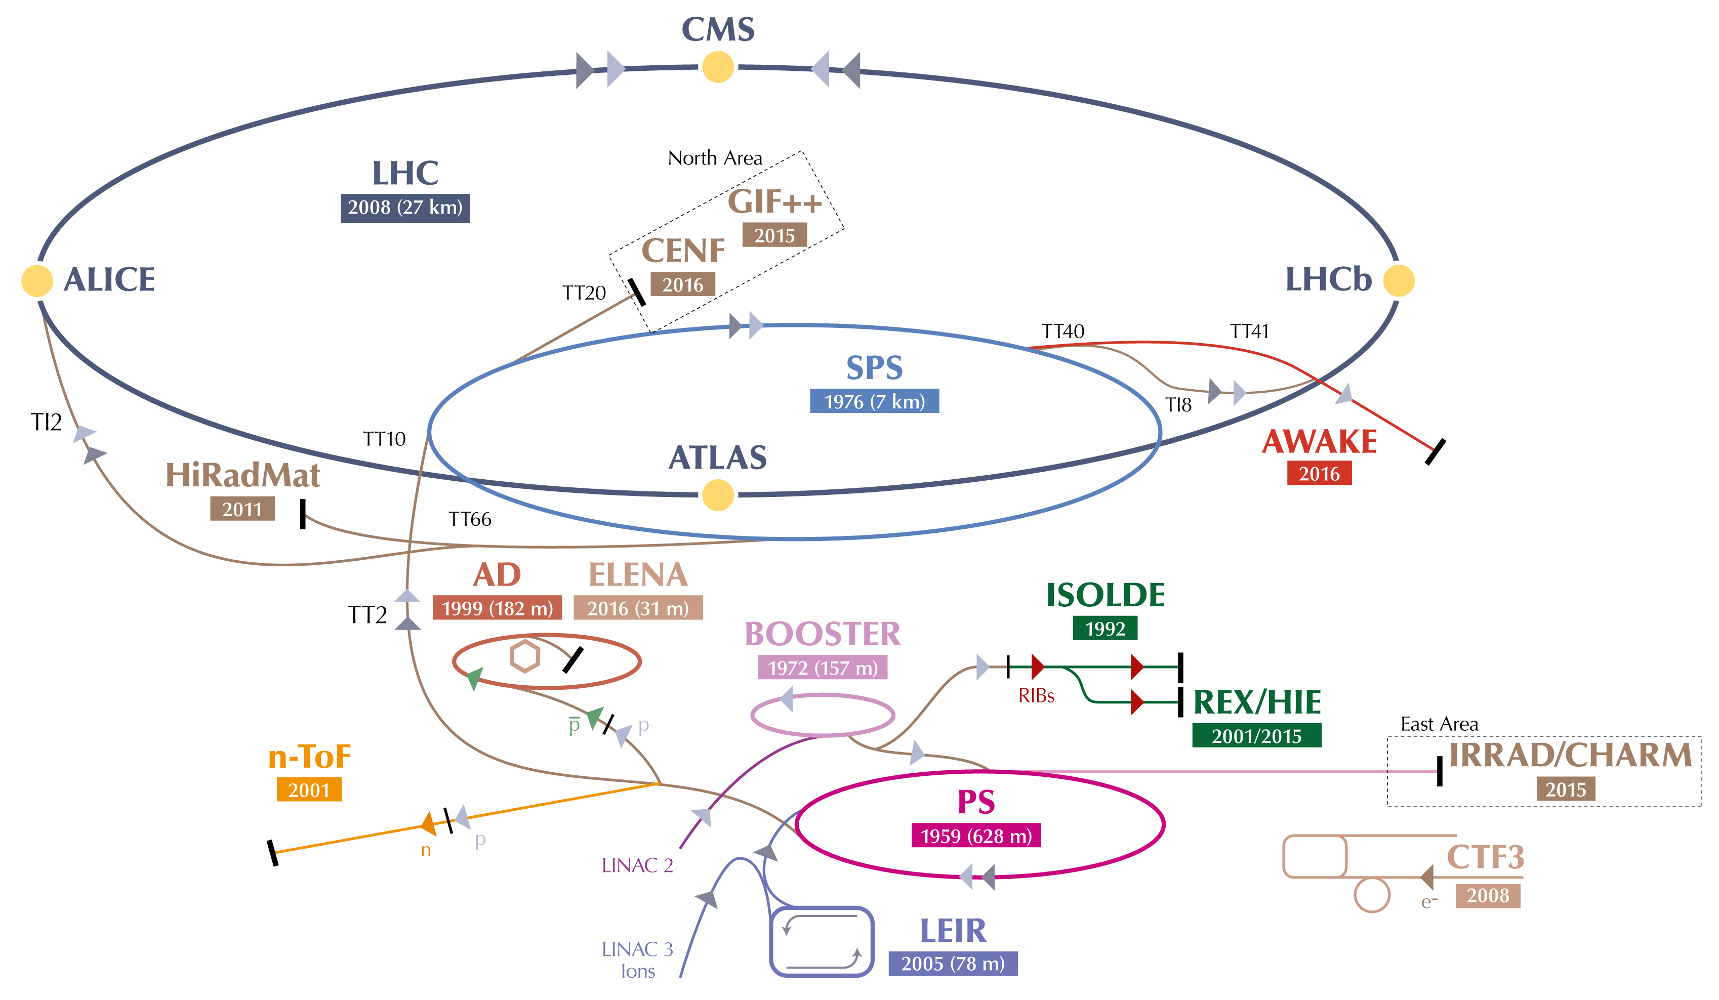
\includegraphics[width=.9\textwidth]{figs/detector/accelerator-complex-small}
  \caption[The CERN accelerator complex.  For LHC collisions, protons are accelerated in the PSB (purple), the PS (magenta), and the SPS (light blue) before entering the LHC ring (dark blue).]{The CERN accelerator complex.  For LHC collisions, protons are accelerated in the PSB (purple), the PS (magenta), and the SPS (light blue) before entering the LHC ring (dark blue)~\cite{2016.accelerator-image}.}
  \label{fig:detector_accelerator_complex}
\end{figure}

In addition to a high center of mass energy, the LHC must also deliver enough data to measure rare processes.
The amount of data collected is measured in terms of \emph{luminosity}.
The instantaneous luminosity $\mathcal{L}$ is defined in terms of the number of events per second $\deriv{R}{t}$ and the production cross section $\sigma_p$:
\begin{equation}
  \mathcal{L} = \frac{1}{\sigma_p}\deriv{R}{t}
  \label{eq:inst_lumi}
\end{equation}
The calculation itself can be quite tricky, as it depends on a number of factors including (but not limited to) the number of particles per bunch, the spread of the beam, and the crossing angle of the beam~\cite{2006.lumi}.

The LHC was originally designed to operate at an instantaneous luminosity of $1.0\times 10^{34}~\textrm{cm}^{-2}\textrm{s}^{-1}$; however, this number was exceeded by the end of the 2016 data taking period, with a peak luminosity of $1.38\times 10^{34}~\textrm{cm}^{-2}\textrm{s}^{-1}$.
This number has been more than doubled by the end of Run 2 in December of 2018~\cite{2019.atlas-lumi-plots}.
The instantaneous luminosity of $pp$ collisions as a function of time in 2015 and 2016 are shown in Figure~\ref{fig:detector_instantaneous_lumi}.
The integrated luminosity is then the time integral of the instantaneous luminosity.
By the end of Run 2 (2015-2018), approximately $140~\textrm{fb}^{-1}$ of $13\tev$ data is available for physics, as shown in Figure~\ref{fig:atlas_integrated_lumi}.
The $36.1~\textrm{fb}^{-1}$ collected during the first two years (2015 and 2016) is used for the analysis later in this thesis.

\begin{figure}[htbp]
  \centering
  \begin{subfigure}[b]{.48\textwidth}
    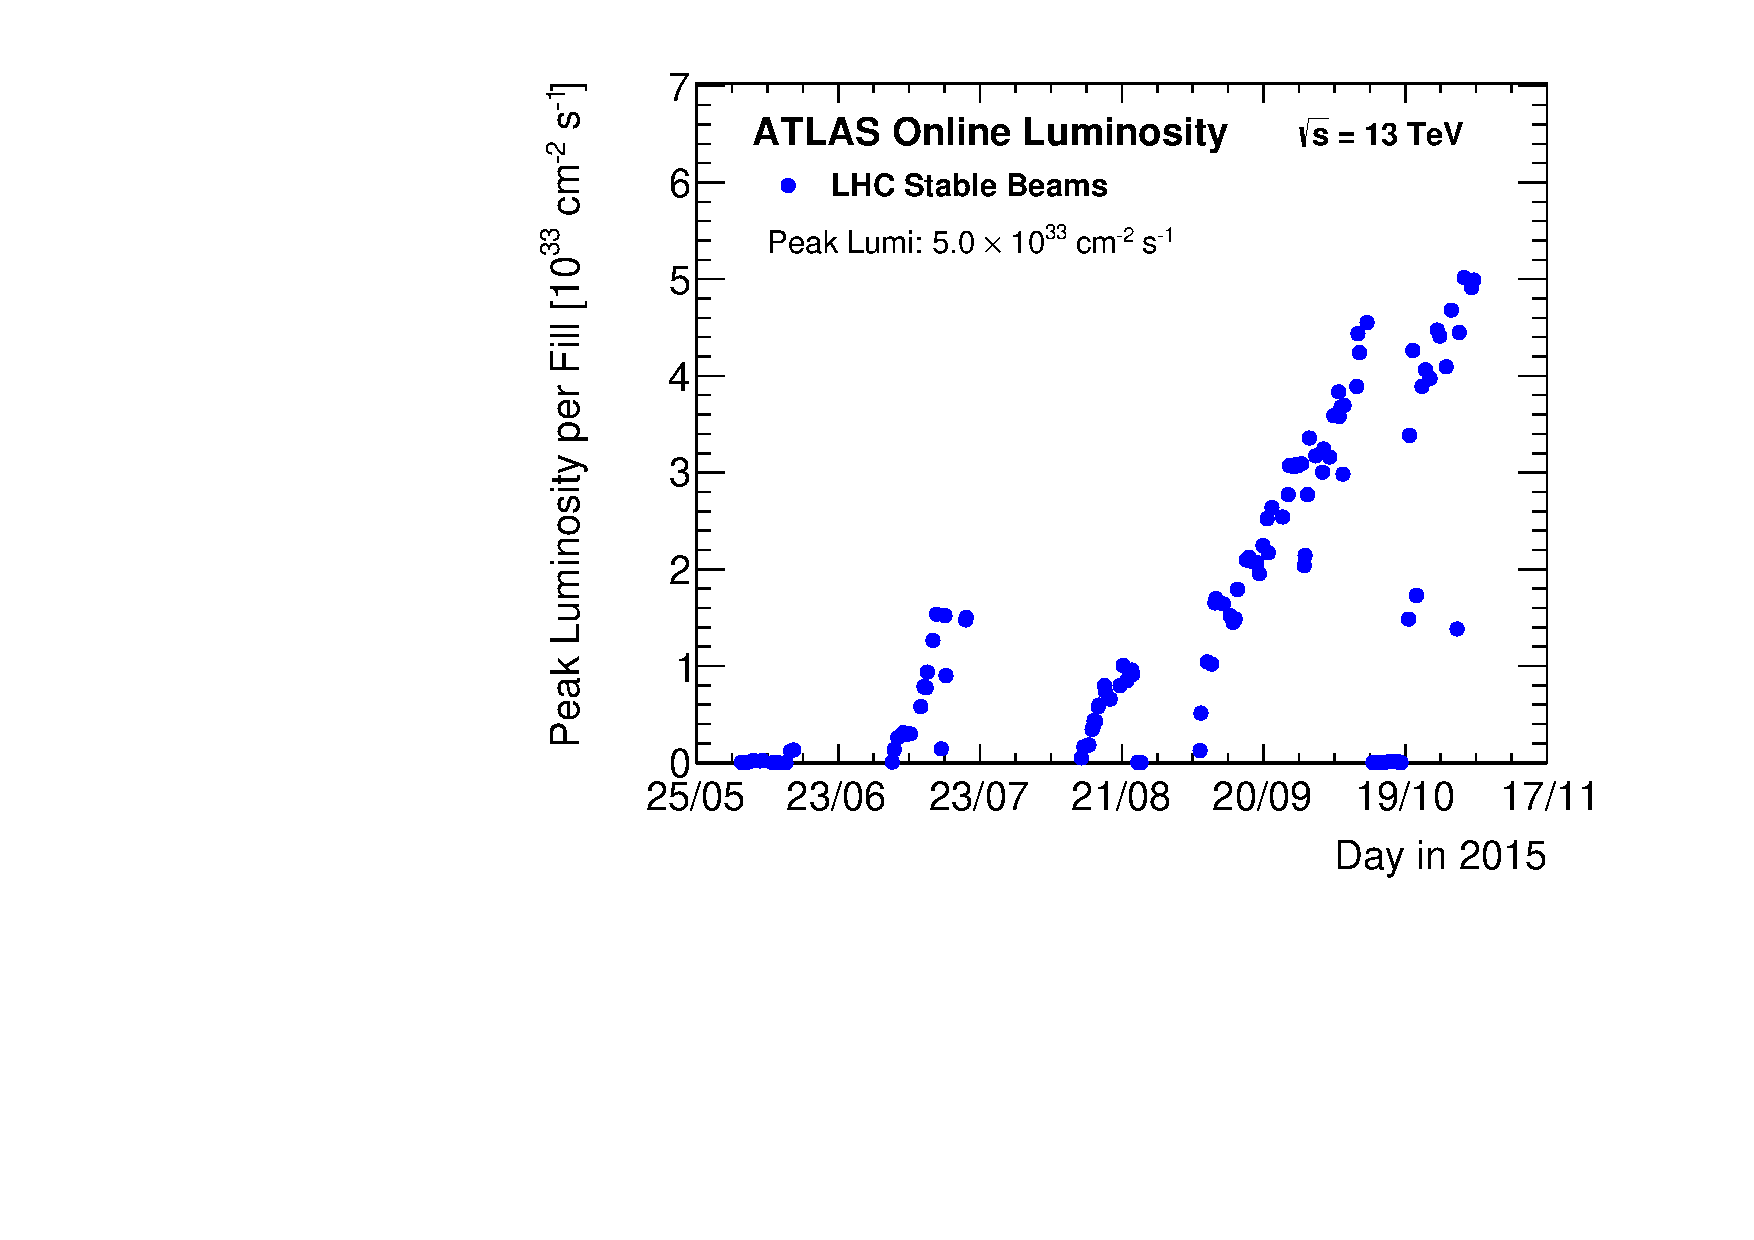
\includegraphics[width=\textwidth]{figs/detector/peakLumiByFill2015}
    \caption{2015}
  \end{subfigure}
  \begin{subfigure}[b]{.48\textwidth}
    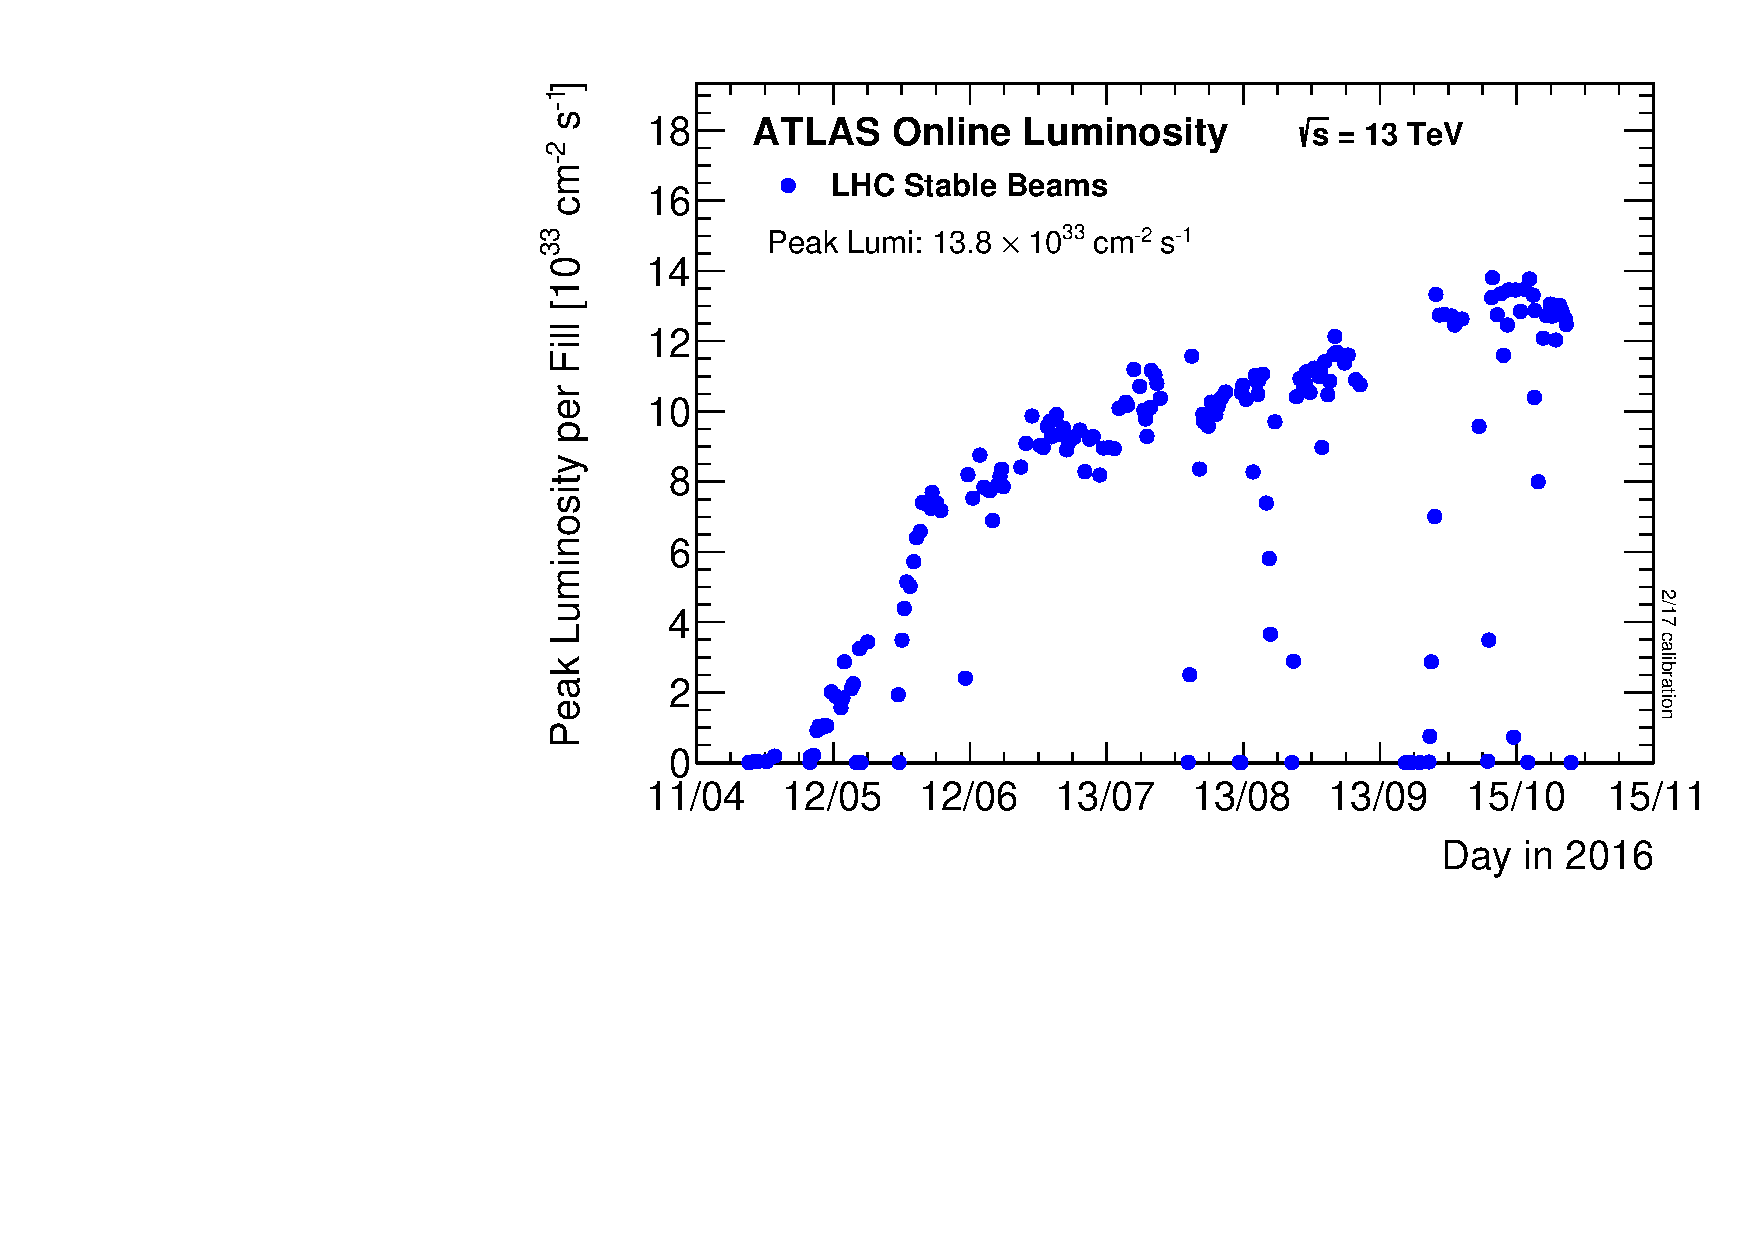
\includegraphics[width=\textwidth]{figs/detector/peakLumiByFill2016}
    \caption{2016}
  \end{subfigure}
  \caption[Peak instantaneous luminosity delivered to ATLAS during $13\tev$ $pp$ data taking as a function of time.]{Peak instantaneous luminosity delivered to ATLAS during $13\tev$ $pp$ data taking as a function of time~\cite{2019.atlas-lumi-plots}.}
  \label{fig:detector_instantaneous_lumi}
\end{figure}

\begin{figure}
  \centering
  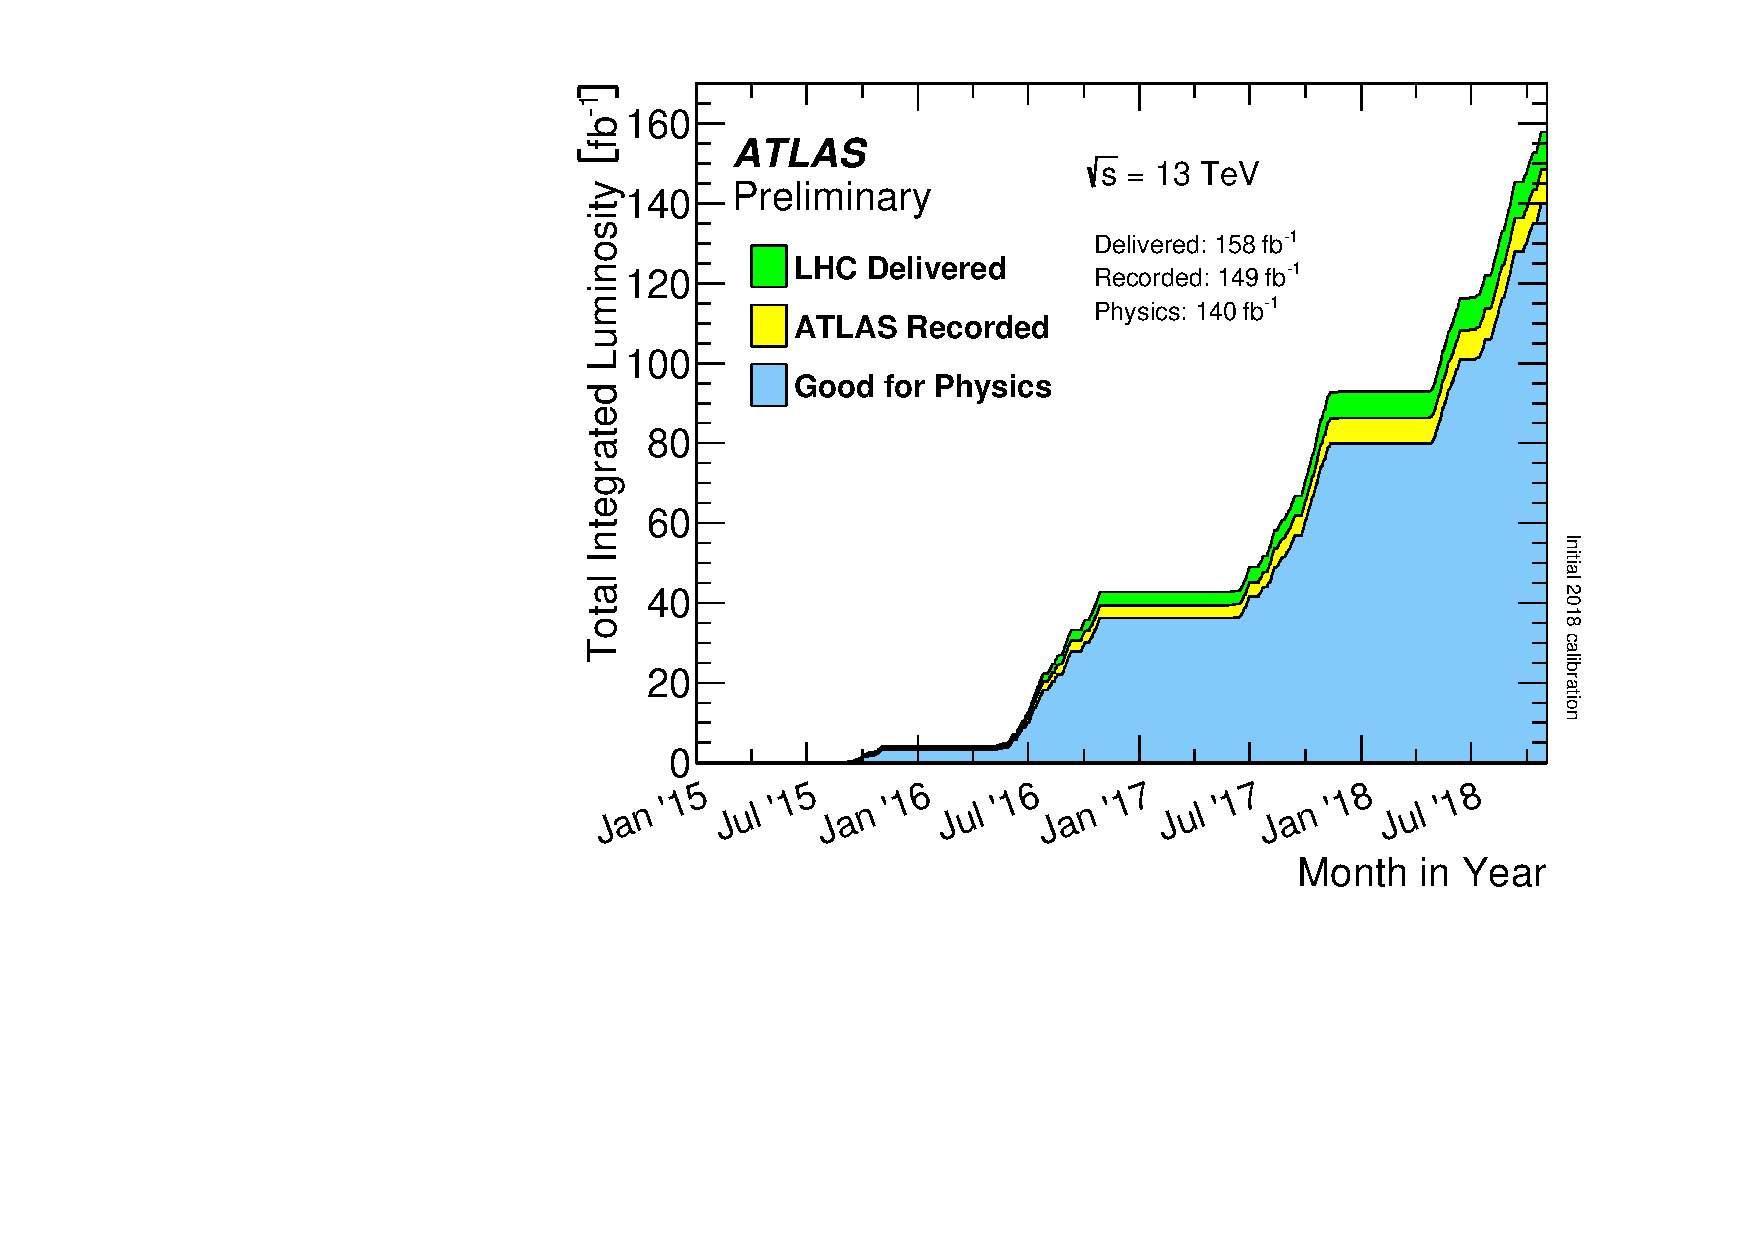
\includegraphics[width=.6\textwidth]{figs/detector/intLumiVsTimeRun2}
  \caption[Integrated luminosity collected by ATLAS as a function of time at $13\tev$ from 2015-2018.]{Integrated luminosity collected by ATLAS as a function of time at $13\tev$ from 2015-2018~\cite{2019.atlas-lumi-plots}.}
  \label{fig:atlas_integrated_lumi}
\end{figure}

Due to the high instantaneous luminosity, more than one $pp$ interaction occurs in a single bunch crossing, referred to as \emph{pileup}.
During the 2016 data taking campaign, the average number of interactions per bunch crossing $<\mu >$ was approximately 24 but has increased to upwards of 37 in 2017 and 2018~\cite{2019.atlas-lumi-plots}.
Figure~\ref{fig:detector_pileup} contains the average $\mu$ for the 2015-2016 data set used for analysis in this thesis.
The high pileup is a challenge for accurately reconstructing an individual collision.

\begin{figure}
  \centering
  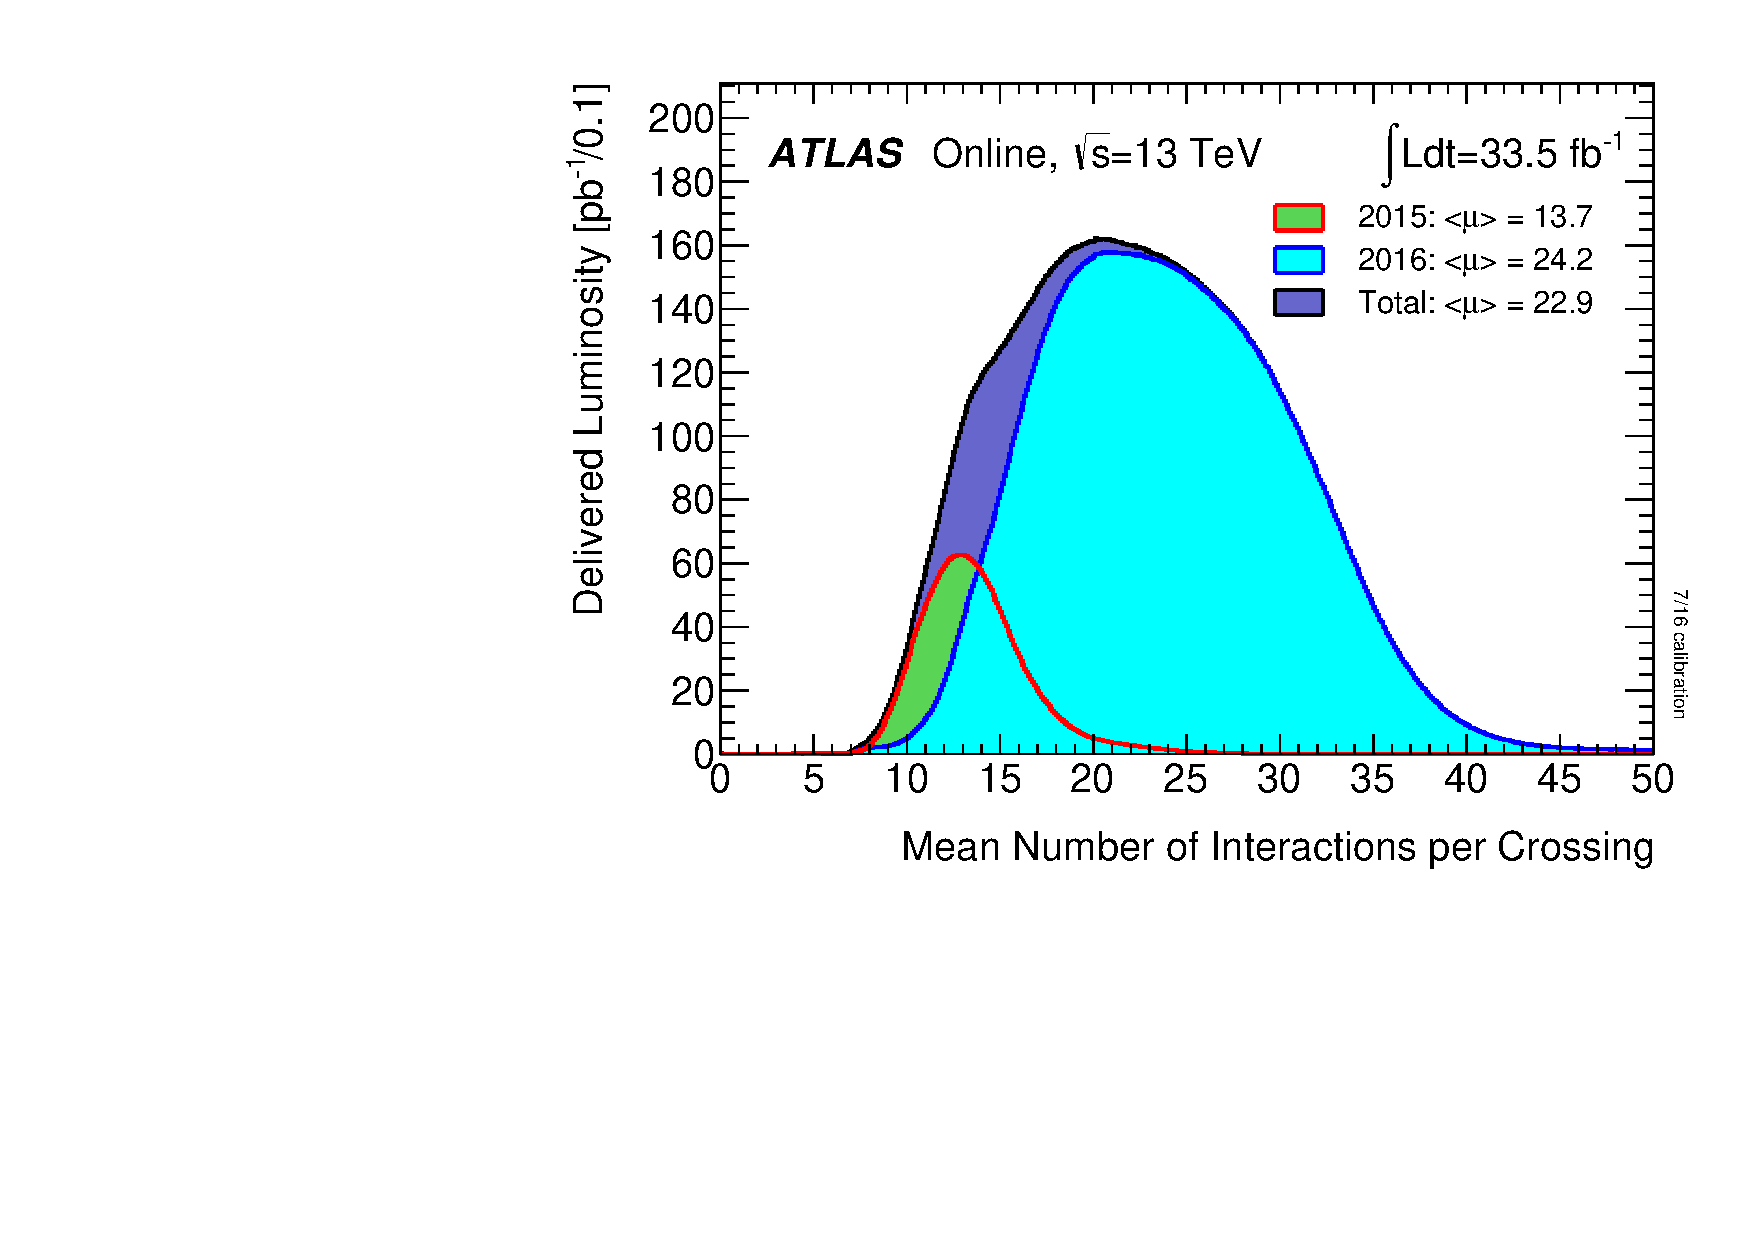
\includegraphics[width=.6\textwidth]{figs/detector/meanInteractionsPerCrossing}
  \caption[Distribution of the mean number of interactions per bunch crossing for the 2015 and 2016 $pp$ collision data at $13\tev$.]{Distribution of the mean number of interactions per bunch crossing for the 2015 and 2016 $pp$ collision data at $13\tev$~\cite{2019.atlas-lumi-plots}.}
  \label{fig:detector_pileup}
\end{figure}


\section{The ATLAS Detector}\label{sec:atlas}
ATLAS is a general-purpose particle detector

% brief overview of detector
% define coordinate system, eta, DeltaR

\begin{figure}[tbp]
  \begin{center}
    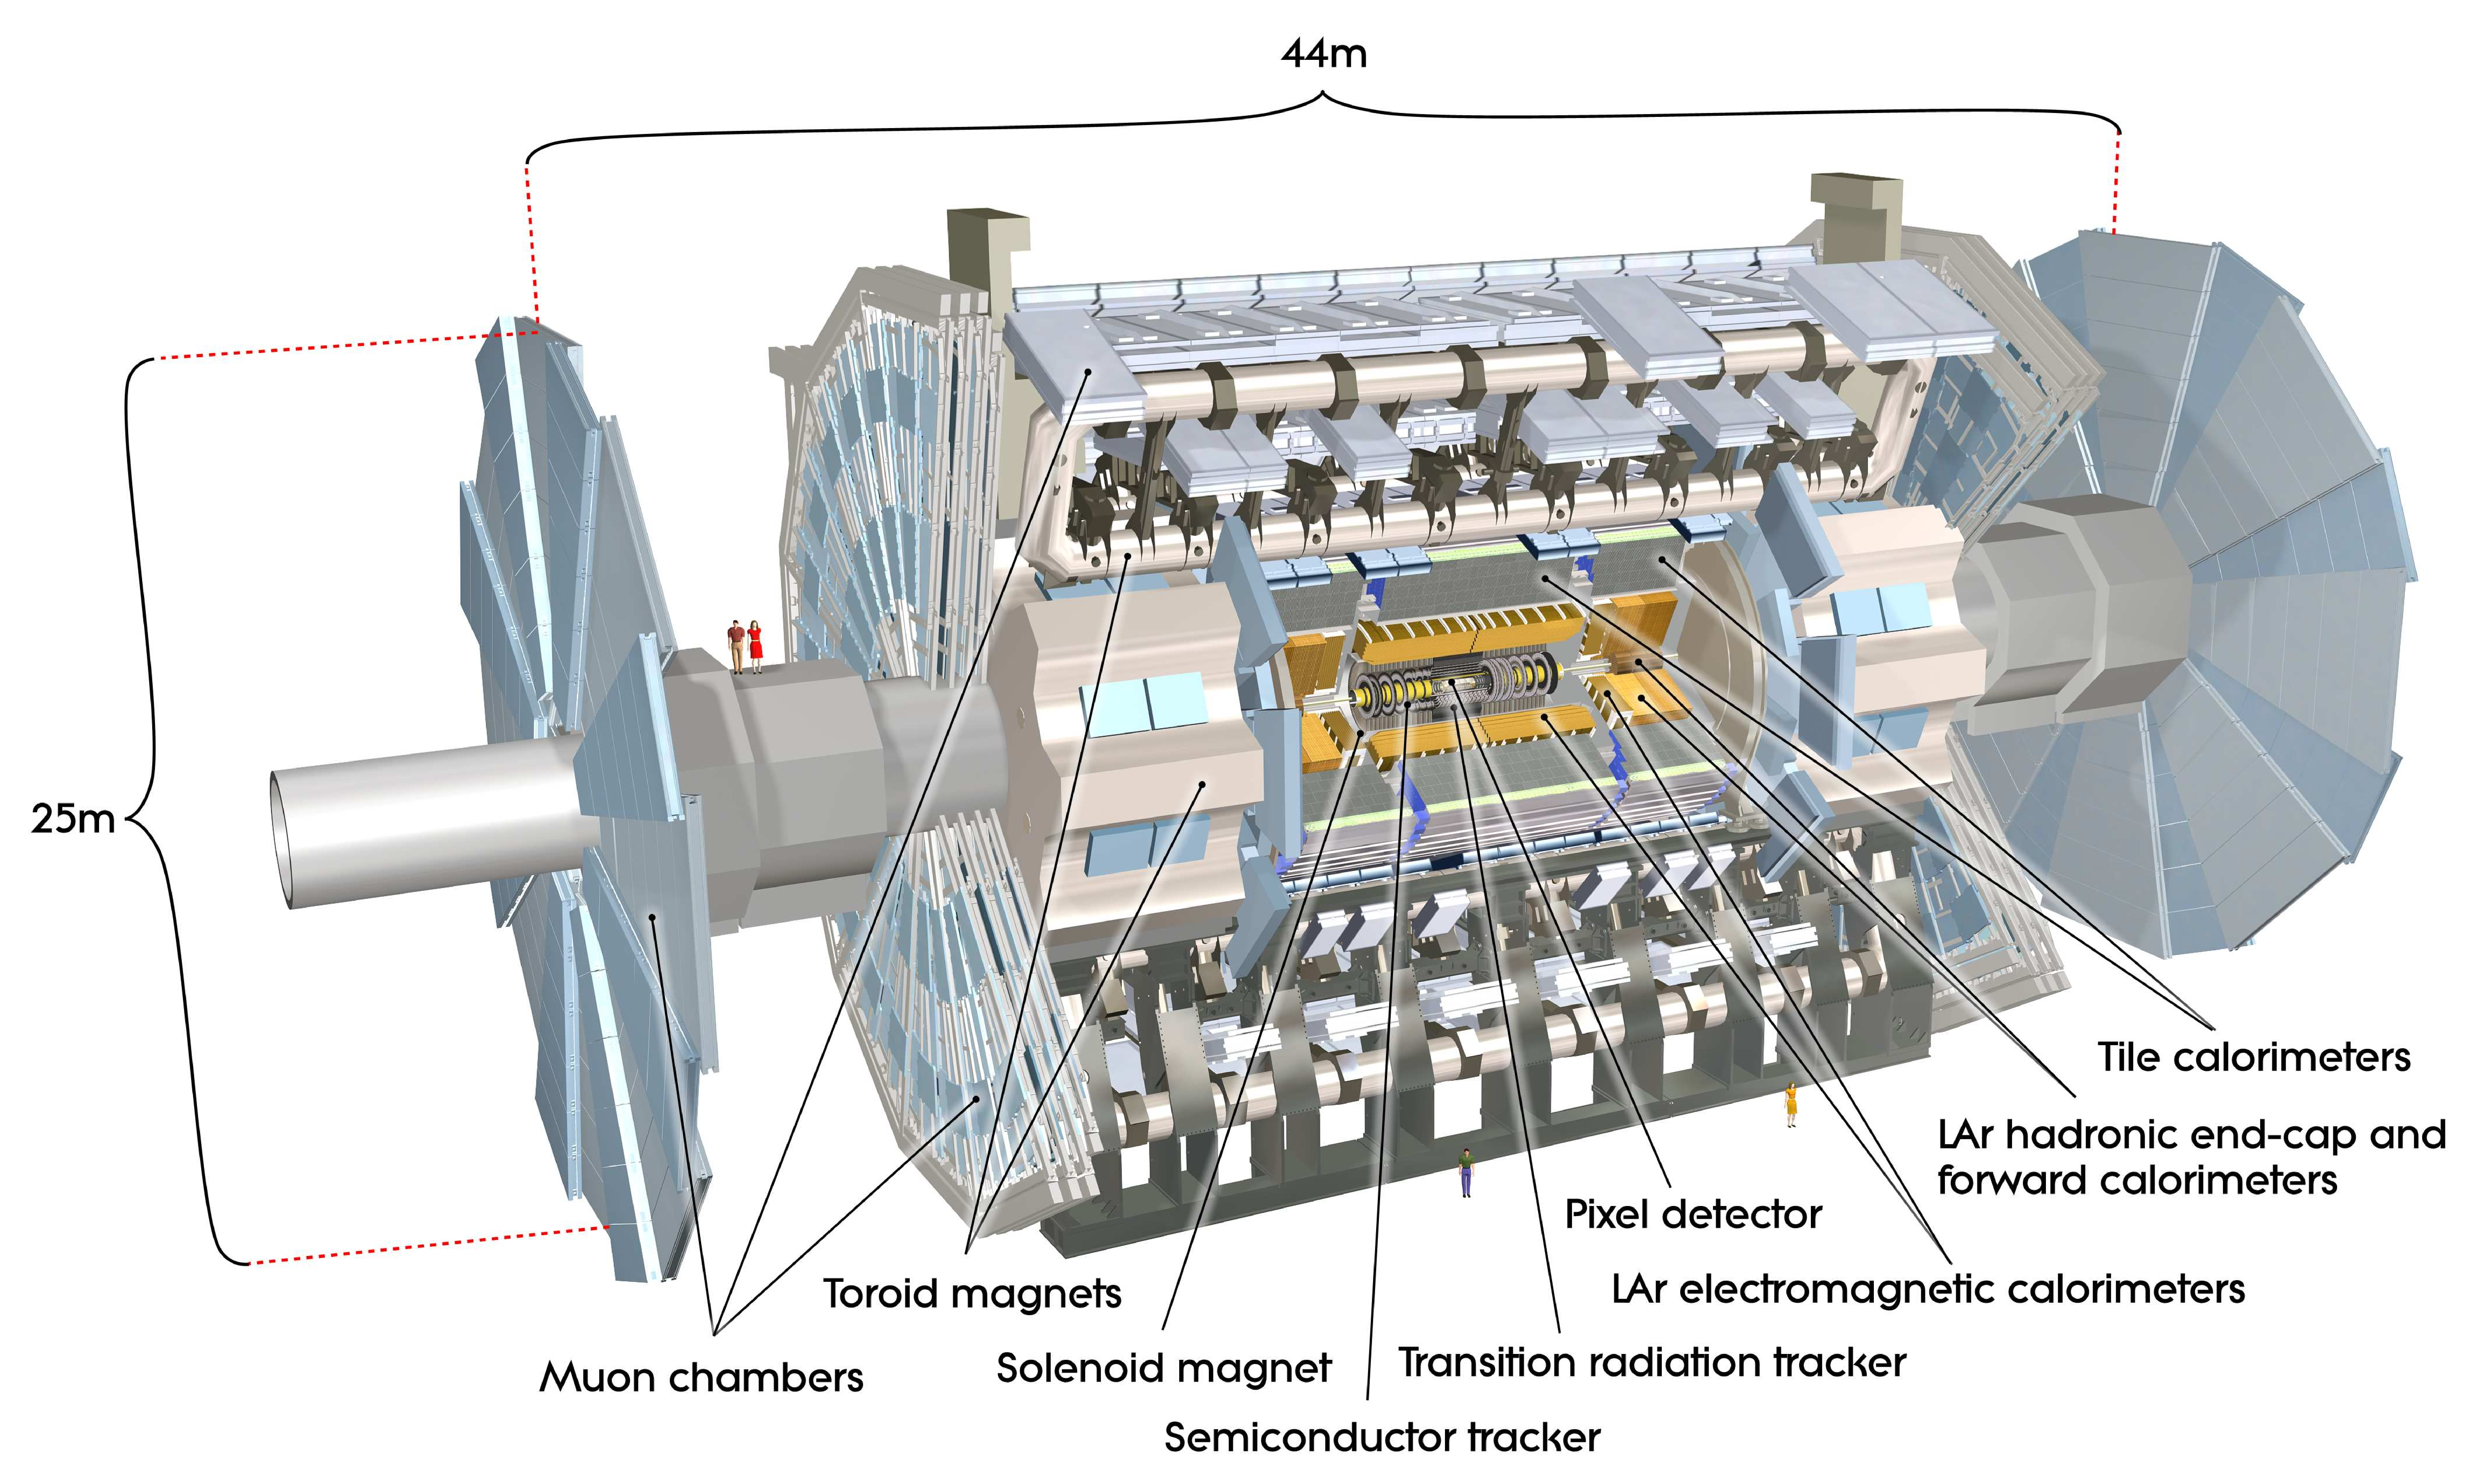
\includegraphics[width=0.98\textwidth]{figs/detector/atlas.pdf}
  \end{center}
  % Optional first argument is what goes into the List of Figures, useful if main caption is long or contains references
  % Second argument here is the actual caption
  \caption[General cut-away view of the ATLAS detector.]
          {General cut-away view of the ATLAS detector \cite{PERF-2007-01}.}
\end{figure}


\subsection{The Inner Detector}\label{sec:id}
The ID~\cite{1997.id-tdr-1, 1997.id-tdr-2} is a tracking system that reconstructs the trajectories of charged particles.
It spans just over a meter in radius, with the innermost layer of sensors at a radius of 33.25~cm from the beam line.
Charged particles traveling through the ID leave \emph{hits} in each sensor they pass through, and a \emph{track} representing the path of the particle is fit to the hits according to the procedure outlined in Section~\ref{detector:track_reconstruction}.
The ID's pseudorapidity coverage extends out to $|\eta| < 2.5$.
A solenoid magnet outside the ID produces a 2~T magnetic field that bends the particles, allowing for their momenta in the direction transverse to the field to be measured according to
\begin{equation}
  \pt = q\cdot B\cdot r\,,
  \label{eq:id_pt}
\end{equation}
where $q$ is the charge of the particle ($\pm 1$), $B$ is the strength of the magnetic field, and $r$ is the radius of the track's curvature.
%The three subdetectors making up the ID are detailed in the following subsections, and additional technical information can be found in~\cite{1997.id-tdr-1, 1997.id-tdr-2}.
A cut-away view of the barrel region of the ID is shown in Figure~\ref{fig:detector_ID}.

\begin{figure}
  \centering
  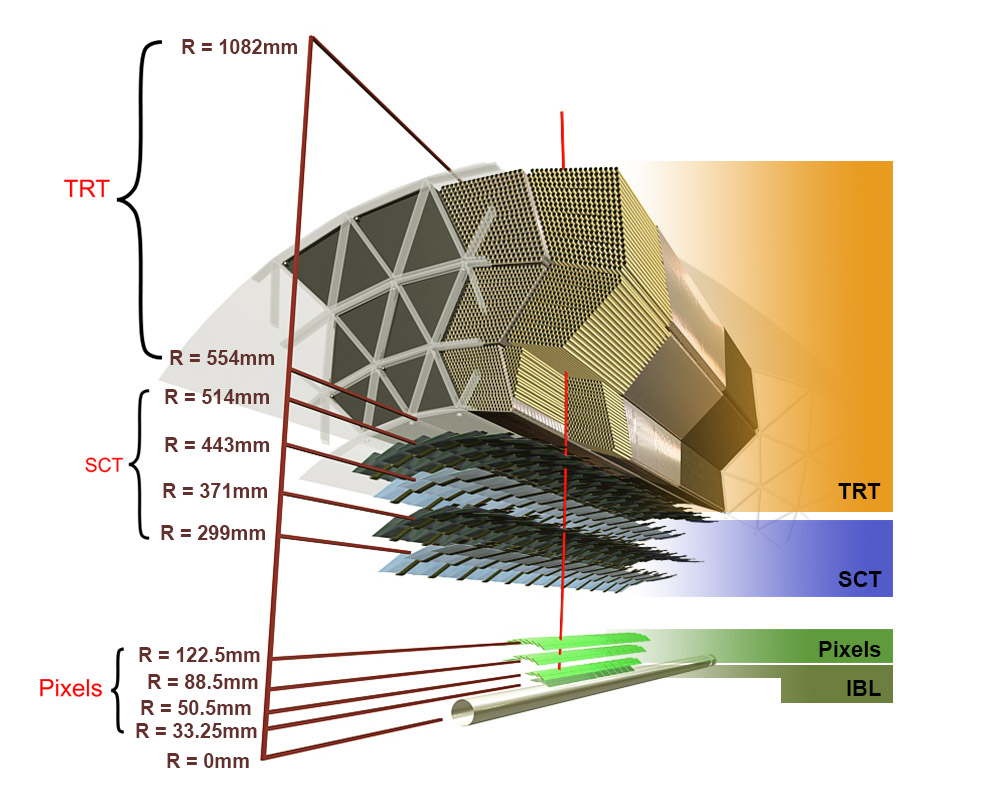
\includegraphics[width=.8\textwidth]{figs/detector/ID}
  \caption{The barrel layers of the Pixel, SCT, and TRT detectors making up the Inner Detector.}
  \label{fig:detector_ID}
\end{figure}

\subsubsection{Pixel Detector} \label{sec:pixel}
The Pixel Detector consists of four cylindrical barrel layers\footnote{For now, the outer three barrel layers will be covered in conjunction with the endcaps; the innermost layer will be described separately.} and three endcap disks on either side.
It is the innermost subdetector of the ID with coverage up to $|\eta| < 2.5$.
The individual sensors measure $50~\mum\times 400~\mum$ and are installed on silicon wafers that make up the layers.
All in all, there are 1744 wafers with 80 million readout channels.
The sensors themselves are silicon semiconducting diodes that provide a signal when a charged particle passes through.
The Pixel Detector has the finest resolution of all the ID subdetectors, at $10~\mum$ in the $r$-$\phi$ plane and $40~\mum$ in the $z$ direction.

During the upgrade period between Run 1 and Run 2, a new innermost layer was added to the Pixel detector barrel: the Insertable B-Layer (IBL)~\cite{2010.ibl-tdr}.
The IBL lies closest to the interaction point, at a radius of 33.25~cm from the beam line, and it is relied upon to provide high-precision measurements close to the interaction point.
Its addition allows better precision in detecting displaced vertices from $b$-jets, for example.
The IBL consists of 280 silicon pixel modules arranged on 14 staves that run parallel to the beam line.
Each stave consists of 12 two-chip planar modules in the middle ($|\eta| < 2.7$) with four 3D sensors~\cite{2015.ibl-3d} on either side ($2.7 < |\eta| < 3.0$).
The IBL's pixel sensors are $50~\mum\times 250~\mum$ in size and have a resolution of $10~\mum$ in $r$-$\phi$ and $75~\mum$ in $z$~\cite{2016.ibl-resolution}.

\subsubsection{Semiconductor Tracker} \label{sec:sct}
The next subdetector of the ID is the SCT, which has four barrel layers and nine endcap disks per side which provide coverage up to $|\eta| < 2.5$.
The SCT operates on the same principle as the Pixel Detector, but the sensitive elements are larger silicon ``strips'' placed on the wafers.
This shape change assists in covering the larger surface area required by the increasing detector radius.
Each detector layer is actually made up of two layers of wafers, placed back-to-back with an angle of 40~mrad between them.
The resolution in the $r$-$\phi$ plane is very fine at $17~\mum$, but, due to the strip shape, the resolution along $z$ is rather poor at $580~\mum$.

\subsubsection{Transition Radiation Tracker} \label{sec:trt}
The outermost component of the ID is the TRT~\cite{2008.trt-tubes, 2008.trt-barrel, 2008.trt-endcap}, which uses a completely different technology from the Pixel and SCT to identify particle hits.
The TRT is unique in that it combines a drift tube tracker with transition radiation detection to assist with electron identification.
The TRT's sensitive elements are drift tubes (referred to as ``straws'') that are 4~mm in diameter and consist of a cylindrical cathode with an anode wire running through the center.
Each straw is filled with a gas mixture including xenon or argon which provides ionizing radiation when high energy particles pass through them.
The resulting electrons drift to the anode and register a voltage, indicating a hit in the detector element.

Between the straws are polyethylene fibers in the barrel and polypropylene foil in the endcaps in order to encourage particles to emit transition radiation photons.
These photons also ionize the gas within the straws, leading to a higher signal.
The TRT takes advantage of the fact that lighter particles are more likely to emit transition radiation by using a ternary output: zero, low-threshold, and high-threshold.
High-threshold hits are generally caused by electrons due to their low mass, and this can help in identifying electron tracks from backgrounds. 

There are over 100,000 straws in the barrel of the TRT, and nearly 250,000 in the endcaps.
The TRT provides pseudorapidity coverage up to $|\eta| < 2.0$ with a resolution in the $r$-$\phi$ plane of $130~\mum$.
Since the drift tubes are insensitive along the direction of the wire, the TRT does not provide a measurement along the $z$ direction.


\subsection{The Calorimeters}\label{sec:calorimeters}
ATLAS utilizes two different calorimeters, the Liquid Argon and Tile Calorimeters~\cite{1996.lar-tdr, 1996.tilecal-tdr}, in order to measure electromagnetic and hadronic objects.
The general principle behind both calorimeters is the same: an incoming particle showers as it passes through, eventually coming to a stop, and the resulting energy deposits are read out.
Both are sampling calorimeters, which consist of alternating layers of a dense material to induce the showering (called the \emph{absorber}) and a second material which measures the energy (called the \emph{active material}).
An advantage to this type of calorimeter is that a very dense absorber can be used in order to produce a shower in a limited space, even if it is unsuitable for measuring the energy from the shower.
However, as a result, some of the energy is deposited in the absorbers, and the total shower energy must be estimated.
ATLAS's calorimeter systems are shown in Figure~\ref{fig:calorimeters}.

\begin{figure}[htbp]
  \centering
  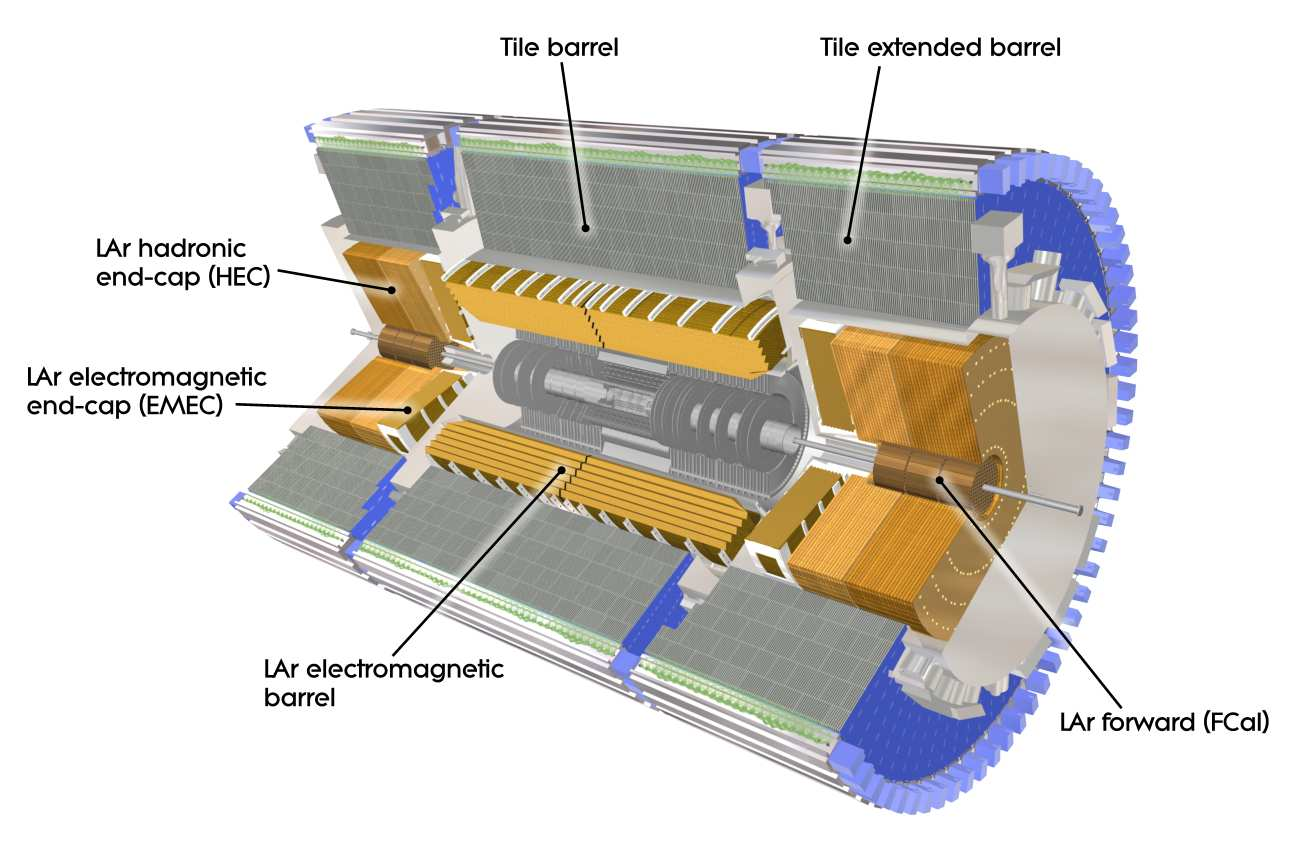
\includegraphics[width=.8\textwidth]{figs/detector/calorimeter}
  \caption[Cut-away view of the ATLAS calorimeter systems.]{Cut-away view of the ATLAS calorimeter systems~\cite{2018.tilecal}.}
  \label{fig:calorimeters}
\end{figure}

Electromagnetic objects, such as electrons and photons, shower via cascades of bremsstrahlung photons and $e^+ e^-$ pairs.
The radiation length $X_0$ is defined as the mean distance over which an electron's energy is reduced to $1/e$ of its original value, or $E(x) = E_{0}e^{-x/X_0}$.
The majority of the shower energy is deposited in the first few radiation lengths.
The longitudinal shower depth scales logarithmically with particle energy, and the transverse shower width is described by the Moli\`{e}re radius\footnote{A cone with a radius equal to the Moli\`{e}re radius ($M_R$) will contain approximately 90\% of the shower energy.  At a radius of $2M_R$, 95\% of the energy will be contained.} of the material.

Hadronic showers (referred to as \emph{jets}) are the result of quarks or gluons which hadronize and shower primarily via the strong interaction.
Hadronic showers are generally wider than the electromagnetic showers described above.
The longitudinal depth of the hadronic shower scales with the nuclear interaction length of the material $\lambda$, defined as the mean distance for the number of particles in a hadronic jet to be reduced to $1/e$ of the initial number.
In addition, about $1/3$ of the shower products are neutral pions $\pi^0$ which decay electromagnetically via the process described above.

%Together, the two calorimeters have pseudorapidity coverage up to $|\eta| < 4.9$.

\subsubsection{Liquid Argon Calorimeter} \label{sec:lar}
The LAr Calorimeter contains four individual calorimeters: the electromagnetic barrel (EMB) and endcaps (EMEC), and the hadronic endcap (HEC) and forward calorimeter (FCal).
The entire calorimeter is surrounded by a cryostat held at a temperature around 90~K.

Focusing on the electromagnetic components first, the EMB covers $|\eta| < 1.475$ and the two EMECs cover $1.375 < |\eta| < 3.2$.
They consist of alternating layers of lead absorber and liquid argon.
The exact thickness of the lead depends on the location within the detector, ranging from 1.1-2.2~mm.
The absorbers are folded into an accordion shape, where the folding angles are varied in order to keep the thickness of the liquid argon gap constant across the barrel (about 2.1~mm).
The electromagnetic calorimeter is thick enough that the minimum number of radiation lengths a particle travels through is $24~X_0$, including the material from other subdetectors.

There are four layers within the EMB and EMEC, including an innermost pre-sampler that helps correct for energy lost before the shower reaches the calorimeter.
The next three layers consist of differently shaped cells successively reducing in granularity.
The first layer consists of narrow strips for fine-grained $\eta$ resolution, while the majority of the shower energy is deposited in the second layer; the third layer captures most of the energy that escapes the previous two.
The accordion shape as well as the sizes of the cells in the EMB are shown in Figure~\ref{fig:lar_accordion}.

\begin{figure}[htbp]
  \centering
  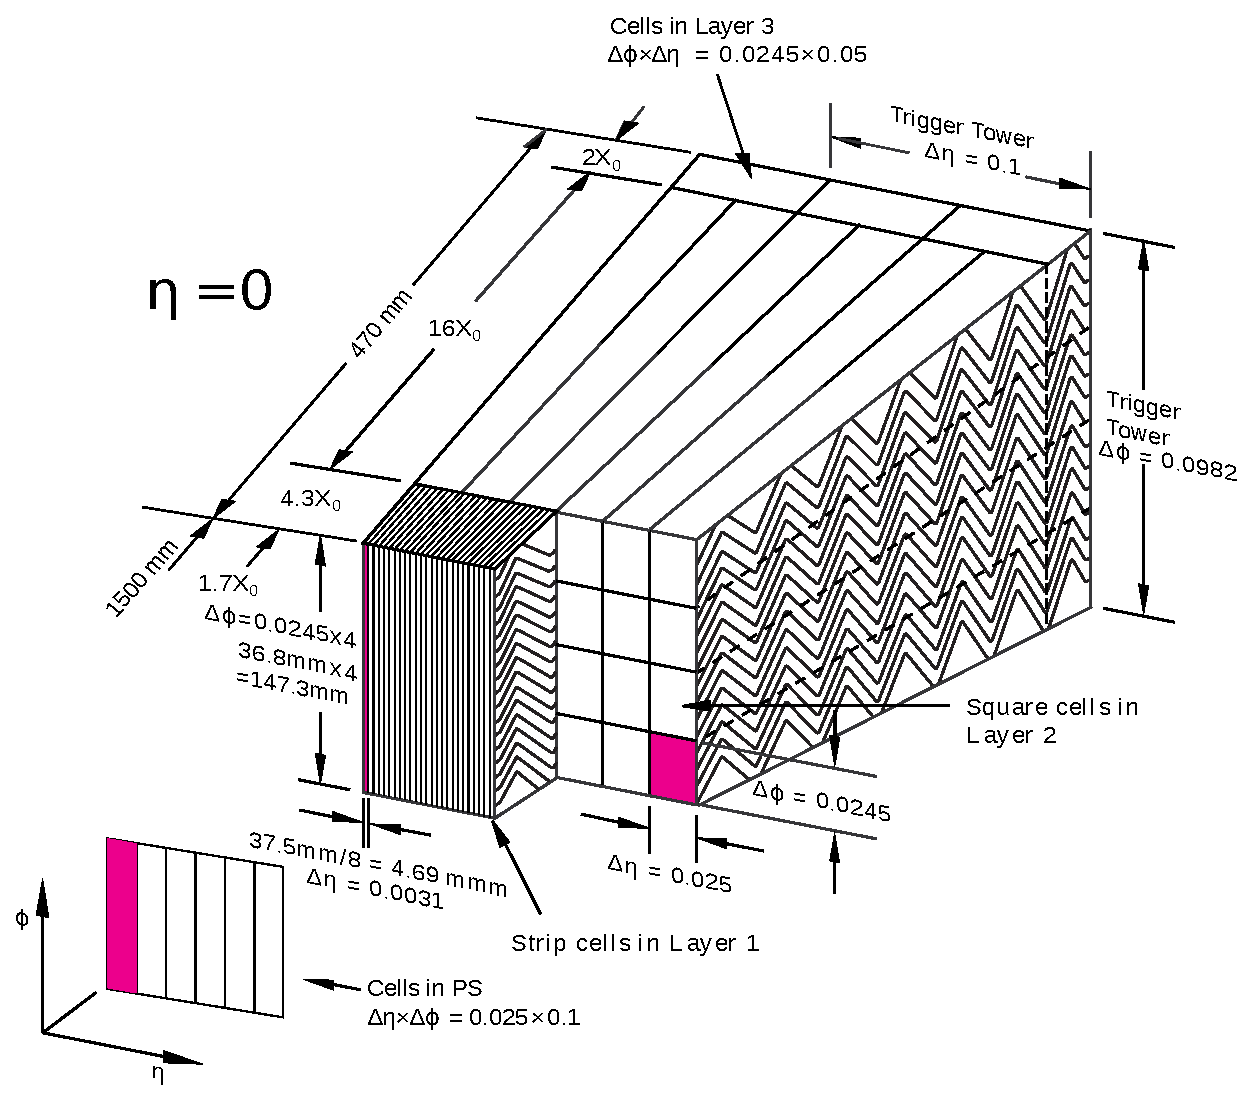
\includegraphics[width=.8\textwidth]{figs/detector/lar_accordion}
  \caption[Diagram of the cells within the LAr barrel.  The accordion structure can be seen in the cut-away view.]{Diagram of the cells within the LAr barrel.  The accordion structure can be seen in the cut-away view~\cite{1996.lar-tdr}.}
  \label{fig:lar_accordion}
\end{figure}

The HEC is located directly behind the EMEC and covers $1.5 < |\eta| < 3.2$.
It uses thick copper plates as the absorber (25~mm in the front wheels and 50~mm in the rear wheels) separated by 8.5~mm gaps filled with liquid argon.
Rather than the accordion shape, the HEC cells are rectangular.

The FCal provides coverage for hadronic jets over the range $3.2 < |\eta| < 4.9$.
Each FCal endcap consists of three layers.
The first is an electromagnetic calorimeter with a copper absorber, while the other two hadronic layers use a tungsten absorber.
Due to the high particle flux entering the FCal, the liquid argon gaps are very narrow, and electrodes are embedded into the absorbers parallel to the beam line.

\subsubsection{Tile Calorimeter}
The TileCal consists of a barrel and two ``extended barrel'' sections which cover the range $|\eta| < 1.7$.
It consists of alternating layers of steel plates and polystyrene scintillator tiles as the absorbers and active material, respectively.
The total thickness of the TileCal is approximately $9~\lambda$.
As the shower passes through the scintillators, photons are emitted that are picked up by wavelength shifting fibers and passed to photomultiplier tubes.
%The resolution of the TileCal is approximately $0.1\times 0.1$ in $\eta$-$\phi$.


\subsection{The Muon Spectrometer}\label{sec:muon_spectrometer}
The outermost subdetector in ATLAS is the Muon Spectrometer~\cite{1997.ms-tdr}.
Due to the high mass of muons compared to electrons, they pass through the calorimeters, necessitating their own detector.
The MS is a high-resolution spectrometer providing tracking for muon reconstruction within $|\eta| < 2.7$.
A set of toroid magets provide an azimuthal magnetic field that bends the muons for momentum measurements, much like in the ID.
Four different technologies are used in the MS:
\begin{itemize}
\item Monitored Drift Tubes (MDT) are used across the entire $\eta$ range for precision measurements of the tracks with a per-hit resolution in the range of 60-80~$\mum$.
These consist of an aluminum tube with an anode wire running through the middle; the tubes are filled with a gas mixture containing argon.
When a muon passes through, the gas is ionized, and the electrons are collected on the wire.
\item Cathode Strip Chambers (CSC) are used for the forward regions of the endcaps (above $|\eta| > 2.0$).
They operate on a similar principle to the MDTs, except they are strips instead of tubes, with a mesh of anode wires running in parallel.
\item Resistive Plate Chambers (RPC) in the barrel are primarily used to provide input for the muon trigger system.
They consist of pairs of plastic resistive plates with a 2~mm gap between them filled with a gas mixture.
Electrodes are attached to the plates, and muons passing through ionize the gas and lead to electric discharges which in turn reduce the potential.
\item Thin Gap Chambers (TGC) are also used for triggering, but for the endcaps.
The TGCs are arranged on circular disks consisting of two rings, and are similar in function to the CSCs but with a different gas mixture.
\end{itemize}


\section{Particle reconstruction}\label{sec:reconstruction}
Particle reconstruction algorithms

\subsubsection{Track reconstruction}\label{detector:track_reconstruction}

\subsubsection{Muon reconstruction}\label{detector:muon_reconstruction}

\subsubsection{Electron reconstruction}\label{detector:electron_reconstruction}

\subsubsection{Jet reconstruction}\label{detector:jet_reconstruction}

